% Options for packages loaded elsewhere
\PassOptionsToPackage{unicode}{hyperref}
\PassOptionsToPackage{hyphens}{url}
%
\documentclass[
]{article}
\usepackage{amsmath,amssymb}
\usepackage{iftex}
\ifPDFTeX
  \usepackage[T1]{fontenc}
  \usepackage[utf8]{inputenc}
  \usepackage{textcomp} % provide euro and other symbols
\else % if luatex or xetex
  \usepackage{unicode-math} % this also loads fontspec
  \defaultfontfeatures{Scale=MatchLowercase}
  \defaultfontfeatures[\rmfamily]{Ligatures=TeX,Scale=1}
\fi
\usepackage{lmodern}
\ifPDFTeX\else
  % xetex/luatex font selection
\fi
% Use upquote if available, for straight quotes in verbatim environments
\IfFileExists{upquote.sty}{\usepackage{upquote}}{}
\IfFileExists{microtype.sty}{% use microtype if available
  \usepackage[]{microtype}
  \UseMicrotypeSet[protrusion]{basicmath} % disable protrusion for tt fonts
}{}
\makeatletter
\@ifundefined{KOMAClassName}{% if non-KOMA class
  \IfFileExists{parskip.sty}{%
    \usepackage{parskip}
  }{% else
    \setlength{\parindent}{0pt}
    \setlength{\parskip}{6pt plus 2pt minus 1pt}}
}{% if KOMA class
  \KOMAoptions{parskip=half}}
\makeatother
\usepackage{xcolor}
\usepackage[margin=1in]{geometry}
\usepackage{color}
\usepackage{fancyvrb}
\newcommand{\VerbBar}{|}
\newcommand{\VERB}{\Verb[commandchars=\\\{\}]}
\DefineVerbatimEnvironment{Highlighting}{Verbatim}{commandchars=\\\{\}}
% Add ',fontsize=\small' for more characters per line
\usepackage{framed}
\definecolor{shadecolor}{RGB}{248,248,248}
\newenvironment{Shaded}{\begin{snugshade}}{\end{snugshade}}
\newcommand{\AlertTok}[1]{\textcolor[rgb]{0.94,0.16,0.16}{#1}}
\newcommand{\AnnotationTok}[1]{\textcolor[rgb]{0.56,0.35,0.01}{\textbf{\textit{#1}}}}
\newcommand{\AttributeTok}[1]{\textcolor[rgb]{0.13,0.29,0.53}{#1}}
\newcommand{\BaseNTok}[1]{\textcolor[rgb]{0.00,0.00,0.81}{#1}}
\newcommand{\BuiltInTok}[1]{#1}
\newcommand{\CharTok}[1]{\textcolor[rgb]{0.31,0.60,0.02}{#1}}
\newcommand{\CommentTok}[1]{\textcolor[rgb]{0.56,0.35,0.01}{\textit{#1}}}
\newcommand{\CommentVarTok}[1]{\textcolor[rgb]{0.56,0.35,0.01}{\textbf{\textit{#1}}}}
\newcommand{\ConstantTok}[1]{\textcolor[rgb]{0.56,0.35,0.01}{#1}}
\newcommand{\ControlFlowTok}[1]{\textcolor[rgb]{0.13,0.29,0.53}{\textbf{#1}}}
\newcommand{\DataTypeTok}[1]{\textcolor[rgb]{0.13,0.29,0.53}{#1}}
\newcommand{\DecValTok}[1]{\textcolor[rgb]{0.00,0.00,0.81}{#1}}
\newcommand{\DocumentationTok}[1]{\textcolor[rgb]{0.56,0.35,0.01}{\textbf{\textit{#1}}}}
\newcommand{\ErrorTok}[1]{\textcolor[rgb]{0.64,0.00,0.00}{\textbf{#1}}}
\newcommand{\ExtensionTok}[1]{#1}
\newcommand{\FloatTok}[1]{\textcolor[rgb]{0.00,0.00,0.81}{#1}}
\newcommand{\FunctionTok}[1]{\textcolor[rgb]{0.13,0.29,0.53}{\textbf{#1}}}
\newcommand{\ImportTok}[1]{#1}
\newcommand{\InformationTok}[1]{\textcolor[rgb]{0.56,0.35,0.01}{\textbf{\textit{#1}}}}
\newcommand{\KeywordTok}[1]{\textcolor[rgb]{0.13,0.29,0.53}{\textbf{#1}}}
\newcommand{\NormalTok}[1]{#1}
\newcommand{\OperatorTok}[1]{\textcolor[rgb]{0.81,0.36,0.00}{\textbf{#1}}}
\newcommand{\OtherTok}[1]{\textcolor[rgb]{0.56,0.35,0.01}{#1}}
\newcommand{\PreprocessorTok}[1]{\textcolor[rgb]{0.56,0.35,0.01}{\textit{#1}}}
\newcommand{\RegionMarkerTok}[1]{#1}
\newcommand{\SpecialCharTok}[1]{\textcolor[rgb]{0.81,0.36,0.00}{\textbf{#1}}}
\newcommand{\SpecialStringTok}[1]{\textcolor[rgb]{0.31,0.60,0.02}{#1}}
\newcommand{\StringTok}[1]{\textcolor[rgb]{0.31,0.60,0.02}{#1}}
\newcommand{\VariableTok}[1]{\textcolor[rgb]{0.00,0.00,0.00}{#1}}
\newcommand{\VerbatimStringTok}[1]{\textcolor[rgb]{0.31,0.60,0.02}{#1}}
\newcommand{\WarningTok}[1]{\textcolor[rgb]{0.56,0.35,0.01}{\textbf{\textit{#1}}}}
\usepackage{graphicx}
\makeatletter
\def\maxwidth{\ifdim\Gin@nat@width>\linewidth\linewidth\else\Gin@nat@width\fi}
\def\maxheight{\ifdim\Gin@nat@height>\textheight\textheight\else\Gin@nat@height\fi}
\makeatother
% Scale images if necessary, so that they will not overflow the page
% margins by default, and it is still possible to overwrite the defaults
% using explicit options in \includegraphics[width, height, ...]{}
\setkeys{Gin}{width=\maxwidth,height=\maxheight,keepaspectratio}
% Set default figure placement to htbp
\makeatletter
\def\fps@figure{htbp}
\makeatother
\setlength{\emergencystretch}{3em} % prevent overfull lines
\providecommand{\tightlist}{%
  \setlength{\itemsep}{0pt}\setlength{\parskip}{0pt}}
\setcounter{secnumdepth}{-\maxdimen} % remove section numbering
\usepackage{booktabs}
\usepackage{longtable}
\usepackage{array}
\usepackage{multirow}
\usepackage{wrapfig}
\usepackage{float}
\usepackage{colortbl}
\usepackage{pdflscape}
\usepackage{tabu}
\usepackage{threeparttable}
\usepackage{threeparttablex}
\usepackage[normalem]{ulem}
\usepackage{makecell}
\usepackage{xcolor}
\ifLuaTeX
  \usepackage{selnolig}  % disable illegal ligatures
\fi
\IfFileExists{bookmark.sty}{\usepackage{bookmark}}{\usepackage{hyperref}}
\IfFileExists{xurl.sty}{\usepackage{xurl}}{} % add URL line breaks if available
\urlstyle{same}
\hypersetup{
  pdftitle={Understanding p values using a simulations},
  pdfauthor={Ian Hussey},
  hidelinks,
  pdfcreator={LaTeX via pandoc}}

\title{Understanding \emph{p} values using a simulations}
\usepackage{etoolbox}
\makeatletter
\providecommand{\subtitle}[1]{% add subtitle to \maketitle
  \apptocmd{\@title}{\par {\large #1 \par}}{}{}
}
\makeatother
\subtitle{Using the example of Welch's independent \emph{t}-test}
\author{Ian Hussey}
\date{12 März, 2024}

\begin{document}
\maketitle

{
\setcounter{tocdepth}{2}
\tableofcontents
}
\begin{Shaded}
\begin{Highlighting}[]
\FunctionTok{library}\NormalTok{(tidyverse)}
\end{Highlighting}
\end{Shaded}

\begin{verbatim}
## -- Attaching core tidyverse packages ------------------------ tidyverse 2.0.0 --
## v dplyr     1.1.4     v readr     2.1.5
## v forcats   1.0.0     v stringr   1.5.1
## v ggplot2   3.5.0     v tibble    3.2.1
## v lubridate 1.9.3     v tidyr     1.3.1
## v purrr     1.0.2     
## -- Conflicts ------------------------------------------ tidyverse_conflicts() --
## x dplyr::filter() masks stats::filter()
## x dplyr::lag()    masks stats::lag()
## i Use the conflicted package (<http://conflicted.r-lib.org/>) to force all conflicts to become errors
\end{verbatim}

\hypertarget{overview-of-tutorial}{%
\section{Overview of tutorial}\label{overview-of-tutorial}}

This lesson focuses on the distributions of \emph{p} values ``under the
null hypothesis'' (i.e., when the null hypothesis is true, aka when the
data generating process is a population model where the effect is zero)
and ``under the alternative hypothesis'' (i.e., when the alternative
hypothesis is true, aka when the data generating process is a population
model where the effect is non-zero).

Without looking into the math, let's use simulations to visualise these
distributions, in order to understand \emph{p} values better.

\hypertarget{plotting-distributions}{%
\section{Plotting distributions}\label{plotting-distributions}}

In the first lesson, we refreshed our knowledge of distributions and
used ggplot to visualise them.

We covered the uniform distribution, where all values between a given
range are equally probable, and the normal distribution, which follows a
normal (gaussian) bell-shaped distribution.

\hypertarget{plot-uniform-distribution}{%
\subsection{Plot uniform distribution}\label{plot-uniform-distribution}}

\begin{Shaded}
\begin{Highlighting}[]
\CommentTok{\# sample values from a uniform distribution, from the range 0 to 1}
\FunctionTok{tibble}\NormalTok{(}\AttributeTok{p =} \FunctionTok{runif}\NormalTok{(}\AttributeTok{n =} \DecValTok{100000}\NormalTok{, }\AttributeTok{min =} \DecValTok{0}\NormalTok{, }\AttributeTok{max =} \DecValTok{1}\NormalTok{)) }\SpecialCharTok{|\textgreater{}}
  \CommentTok{\# create a decision for each value, with values \textless{} .05 labelled as "significant" and those \textgreater{} .05 as "non{-}significant"}
  \FunctionTok{mutate}\NormalTok{(}\AttributeTok{decision =} \FunctionTok{ifelse}\NormalTok{(p }\SpecialCharTok{\textless{}}\NormalTok{ .}\DecValTok{05}\NormalTok{, }\StringTok{"significant"}\NormalTok{, }\StringTok{"non{-}significant"}\NormalTok{)) }\SpecialCharTok{|\textgreater{}}
  \CommentTok{\# plot a histogram of these values, with the fill contingent on the the decision}
  \FunctionTok{ggplot}\NormalTok{(}\FunctionTok{aes}\NormalTok{(p, }\AttributeTok{fill =}\NormalTok{ decision)) }\SpecialCharTok{+}
  \FunctionTok{geom\_histogram}\NormalTok{(}\AttributeTok{binwidth =} \FloatTok{0.05}\NormalTok{, }\AttributeTok{boundary =} \DecValTok{0}\NormalTok{) }\SpecialCharTok{+}
  \FunctionTok{scale\_fill\_viridis\_d}\NormalTok{(}\AttributeTok{option =} \StringTok{"mako"}\NormalTok{, }\AttributeTok{begin =} \FloatTok{0.3}\NormalTok{, }\AttributeTok{end =} \FloatTok{0.7}\NormalTok{, }\AttributeTok{direction =} \SpecialCharTok{{-}}\DecValTok{1}\NormalTok{) }\SpecialCharTok{+}
  \FunctionTok{scale\_x\_continuous}\NormalTok{(}\AttributeTok{labels =} \FunctionTok{c}\NormalTok{(}\DecValTok{0}\NormalTok{, }\FloatTok{0.05}\NormalTok{, }\FloatTok{0.25}\NormalTok{, }\FloatTok{0.50}\NormalTok{, }\FloatTok{0.75}\NormalTok{, }\FloatTok{1.0}\NormalTok{),}
                     \AttributeTok{breaks =} \FunctionTok{c}\NormalTok{(}\DecValTok{0}\NormalTok{, }\FloatTok{0.05}\NormalTok{, }\FloatTok{0.25}\NormalTok{, }\FloatTok{0.50}\NormalTok{, }\FloatTok{0.75}\NormalTok{, }\FloatTok{1.0}\NormalTok{), }
                     \AttributeTok{limits =} \FunctionTok{c}\NormalTok{(}\DecValTok{0}\NormalTok{, }\DecValTok{1}\NormalTok{)) }\SpecialCharTok{+}
  \FunctionTok{theme\_linedraw}\NormalTok{() }\SpecialCharTok{+}
  \FunctionTok{ylab}\NormalTok{(}\StringTok{"Frequency"}\NormalTok{)}
\end{Highlighting}
\end{Shaded}

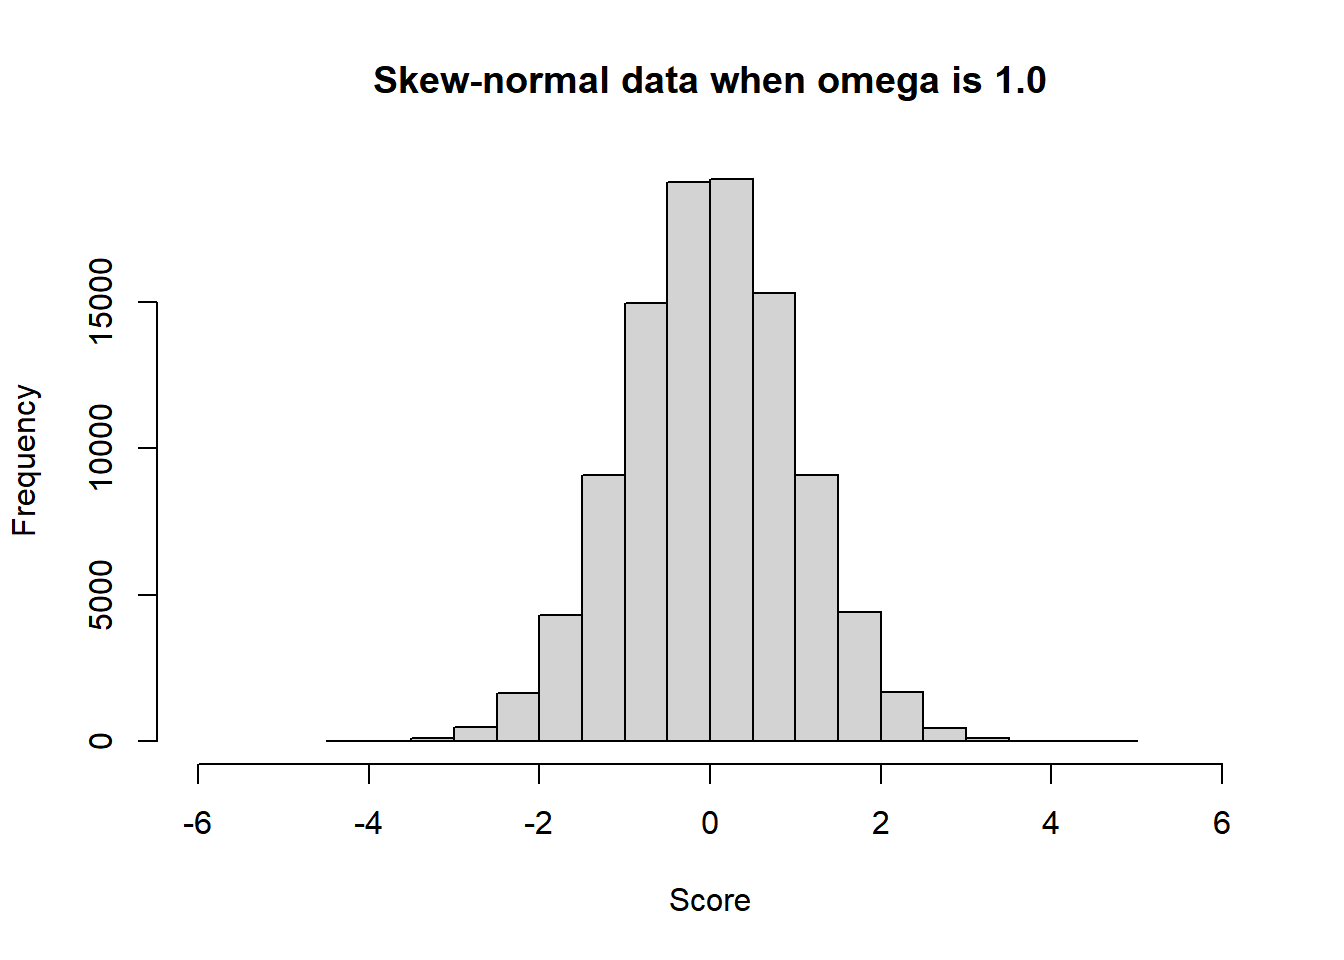
\includegraphics{3_p_values__lesson_files/figure-latex/unnamed-chunk-2-1.pdf}

\begin{itemize}
\tightlist
\item
  Note that this plot labels the x axis as \emph{p} values, but the
  results are not actually \emph{p} values yet: it's just data drawn
  from a uniform distribution.
\end{itemize}

\hypertarget{plot-normal-distribution}{%
\subsection{Plot normal distribution}\label{plot-normal-distribution}}

With the constraint that all values must be within the range {[}0, 1{]}
to mimic \emph{p} values.

\begin{Shaded}
\begin{Highlighting}[]
\CommentTok{\# sample values from a uniform distribution, from the range 0 to 1}
\FunctionTok{tibble}\NormalTok{(}\AttributeTok{p =} \FunctionTok{rnorm}\NormalTok{(}\AttributeTok{n =} \DecValTok{100000}\NormalTok{, }\AttributeTok{mean =} \FloatTok{0.5}\NormalTok{, }\AttributeTok{sd =} \FloatTok{0.25}\NormalTok{)) }\SpecialCharTok{|\textgreater{}}
  \CommentTok{\# drop all values that are outside the range [0, 1] to mimic p values}
  \FunctionTok{filter}\NormalTok{(p }\SpecialCharTok{\textgreater{}=} \DecValTok{0} \SpecialCharTok{\&}\NormalTok{ p }\SpecialCharTok{\textless{}=} \DecValTok{1}\NormalTok{) }\SpecialCharTok{|\textgreater{}}
  \CommentTok{\# create a decision for each value, with values \textless{} .05 labelled as "significant" and those \textgreater{} .05 as "non{-}significant"}
  \FunctionTok{mutate}\NormalTok{(}\AttributeTok{decision =} \FunctionTok{ifelse}\NormalTok{(p }\SpecialCharTok{\textless{}}\NormalTok{ .}\DecValTok{05}\NormalTok{, }\StringTok{"significant"}\NormalTok{, }\StringTok{"non{-}significant"}\NormalTok{)) }\SpecialCharTok{|\textgreater{}}
  \CommentTok{\# plot a histogram of these values, with the fill contingent on the the decision}
  \FunctionTok{ggplot}\NormalTok{(}\FunctionTok{aes}\NormalTok{(p, }\AttributeTok{fill =}\NormalTok{ decision)) }\SpecialCharTok{+}
  \FunctionTok{geom\_histogram}\NormalTok{(}\AttributeTok{binwidth =} \FloatTok{0.05}\NormalTok{, }\AttributeTok{boundary =} \DecValTok{0}\NormalTok{) }\SpecialCharTok{+}
  \FunctionTok{scale\_fill\_viridis\_d}\NormalTok{(}\AttributeTok{option =} \StringTok{"mako"}\NormalTok{, }\AttributeTok{begin =} \FloatTok{0.3}\NormalTok{, }\AttributeTok{end =} \FloatTok{0.7}\NormalTok{, }\AttributeTok{direction =} \SpecialCharTok{{-}}\DecValTok{1}\NormalTok{) }\SpecialCharTok{+}
  \FunctionTok{scale\_x\_continuous}\NormalTok{(}\AttributeTok{labels =} \FunctionTok{c}\NormalTok{(}\DecValTok{0}\NormalTok{, }\FloatTok{0.05}\NormalTok{, }\FloatTok{0.25}\NormalTok{, }\FloatTok{0.50}\NormalTok{, }\FloatTok{0.75}\NormalTok{, }\FloatTok{1.0}\NormalTok{),}
                     \AttributeTok{breaks =} \FunctionTok{c}\NormalTok{(}\DecValTok{0}\NormalTok{, }\FloatTok{0.05}\NormalTok{, }\FloatTok{0.25}\NormalTok{, }\FloatTok{0.50}\NormalTok{, }\FloatTok{0.75}\NormalTok{, }\FloatTok{1.0}\NormalTok{), }
                     \AttributeTok{limits =} \FunctionTok{c}\NormalTok{(}\DecValTok{0}\NormalTok{, }\DecValTok{1}\NormalTok{)) }\SpecialCharTok{+}
  \FunctionTok{theme\_linedraw}\NormalTok{() }\SpecialCharTok{+}
  \FunctionTok{ylab}\NormalTok{(}\StringTok{"Frequency"}\NormalTok{)}
\end{Highlighting}
\end{Shaded}

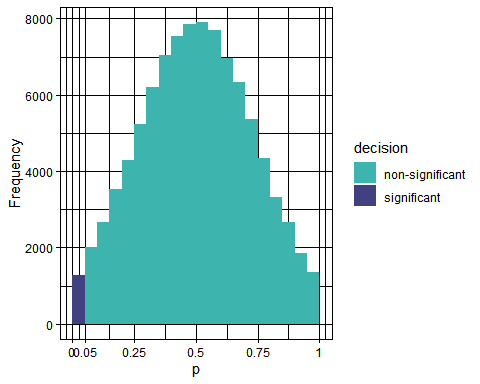
\includegraphics{3_p_values__lesson_files/figure-latex/unnamed-chunk-3-1.pdf}

\begin{itemize}
\tightlist
\item
  Again, note that this plot labels the x axis as \emph{p} values, but
  the results are not actually \emph{p} values yet: it's just data drawn
  from a normal distribution.
\end{itemize}

\hypertarget{coding-rule-dont-repeat-yourself-practice-writing-functions}{%
\subsection{Coding rule: Don't repeat yourself / practice writing
functions}\label{coding-rule-dont-repeat-yourself-practice-writing-functions}}

A key rule when writing code is, in general, \emph{don't repeat
yourself}.

If I want to change the way the above plots are made, or make new ones,
I would need to change the code for each one. Equally, if I want do make
several more plots like this I would need to repeat the code many times.
Every time you copy and paste code like this, it's another opportunity
to make a mistake, eg. to forget to update a parameter somewhere. A good
way to avoid this is to write a function to do it for you, and call this
function as you need it.

Let's use this as an opportunity to practice writing functions, as
you'll need to get good at this for the data generation and analysis
functions you use in simulations anyway.

Let's assume that the simulated data is already generated, and that we
just want to plot it. I therefore move all the code for plotting inside
the new function, and pass data to it via the \texttt{data} parameter.

\begin{Shaded}
\begin{Highlighting}[]
\NormalTok{plot\_p\_values }\OtherTok{\textless{}{-}} \ControlFlowTok{function}\NormalTok{(data)\{ }\CommentTok{\# assumes that data is a data frame with a column "p"}
\NormalTok{  data }\SpecialCharTok{|\textgreater{}}
    \FunctionTok{mutate}\NormalTok{(}\AttributeTok{decision =} \FunctionTok{ifelse}\NormalTok{(p }\SpecialCharTok{\textless{}}\NormalTok{ .}\DecValTok{05}\NormalTok{, }\StringTok{"significant"}\NormalTok{, }\StringTok{"non{-}significant"}\NormalTok{)) }\SpecialCharTok{|\textgreater{}}
    \FunctionTok{ggplot}\NormalTok{(}\FunctionTok{aes}\NormalTok{(p, }\AttributeTok{fill =}\NormalTok{ decision)) }\SpecialCharTok{+}
    \FunctionTok{geom\_histogram}\NormalTok{(}\AttributeTok{binwidth =} \FloatTok{0.05}\NormalTok{, }\AttributeTok{boundary =} \DecValTok{0}\NormalTok{) }\SpecialCharTok{+}
    \FunctionTok{scale\_fill\_viridis\_d}\NormalTok{(}\AttributeTok{option =} \StringTok{"mako"}\NormalTok{, }\AttributeTok{begin =} \FloatTok{0.3}\NormalTok{, }\AttributeTok{end =} \FloatTok{0.7}\NormalTok{, }\AttributeTok{direction =} \SpecialCharTok{{-}}\DecValTok{1}\NormalTok{) }\SpecialCharTok{+}
    \FunctionTok{scale\_x\_continuous}\NormalTok{(}\AttributeTok{labels =} \FunctionTok{c}\NormalTok{(}\DecValTok{0}\NormalTok{, }\FloatTok{0.05}\NormalTok{, }\FloatTok{0.25}\NormalTok{, }\FloatTok{0.50}\NormalTok{, }\FloatTok{0.75}\NormalTok{, }\FloatTok{1.0}\NormalTok{),}
                       \AttributeTok{breaks =} \FunctionTok{c}\NormalTok{(}\DecValTok{0}\NormalTok{, }\FloatTok{0.05}\NormalTok{, }\FloatTok{0.25}\NormalTok{, }\FloatTok{0.50}\NormalTok{, }\FloatTok{0.75}\NormalTok{, }\FloatTok{1.0}\NormalTok{), }
                       \AttributeTok{limits =} \FunctionTok{c}\NormalTok{(}\DecValTok{0}\NormalTok{, }\DecValTok{1}\NormalTok{)) }\SpecialCharTok{+}
    \FunctionTok{theme\_linedraw}\NormalTok{() }\SpecialCharTok{+}
    \FunctionTok{ylab}\NormalTok{(}\StringTok{"Frequency"}\NormalTok{)}
\NormalTok{\}}
\end{Highlighting}
\end{Shaded}

We can then use the function to plot any suitable data, as long as it
(a) has a variable named \texttt{p} and (b) has some values between 0
and 1.

We can even plot data from other distributions, such as the Beta
distribution. The beta distribution can be useful to create fake
\emph{p}-values, as it is bounded {[}0, 1{]} and can generate data that
is anywhere between uniform, normal, or skewed depending on the values
you use for its \(\alpha\) (\texttt{shape1}) and \(\beta\)
(\texttt{shape2}) parameters.

For example:

\begin{Shaded}
\begin{Highlighting}[]
\FunctionTok{tibble}\NormalTok{(}\AttributeTok{p =} \FunctionTok{rbeta}\NormalTok{(}\AttributeTok{n =} \DecValTok{100000}\NormalTok{, }\AttributeTok{shape1 =} \DecValTok{5}\NormalTok{, }\AttributeTok{shape2 =} \DecValTok{5}\NormalTok{)) }\SpecialCharTok{|\textgreater{}}
  \FunctionTok{plot\_p\_values}\NormalTok{()}
\end{Highlighting}
\end{Shaded}

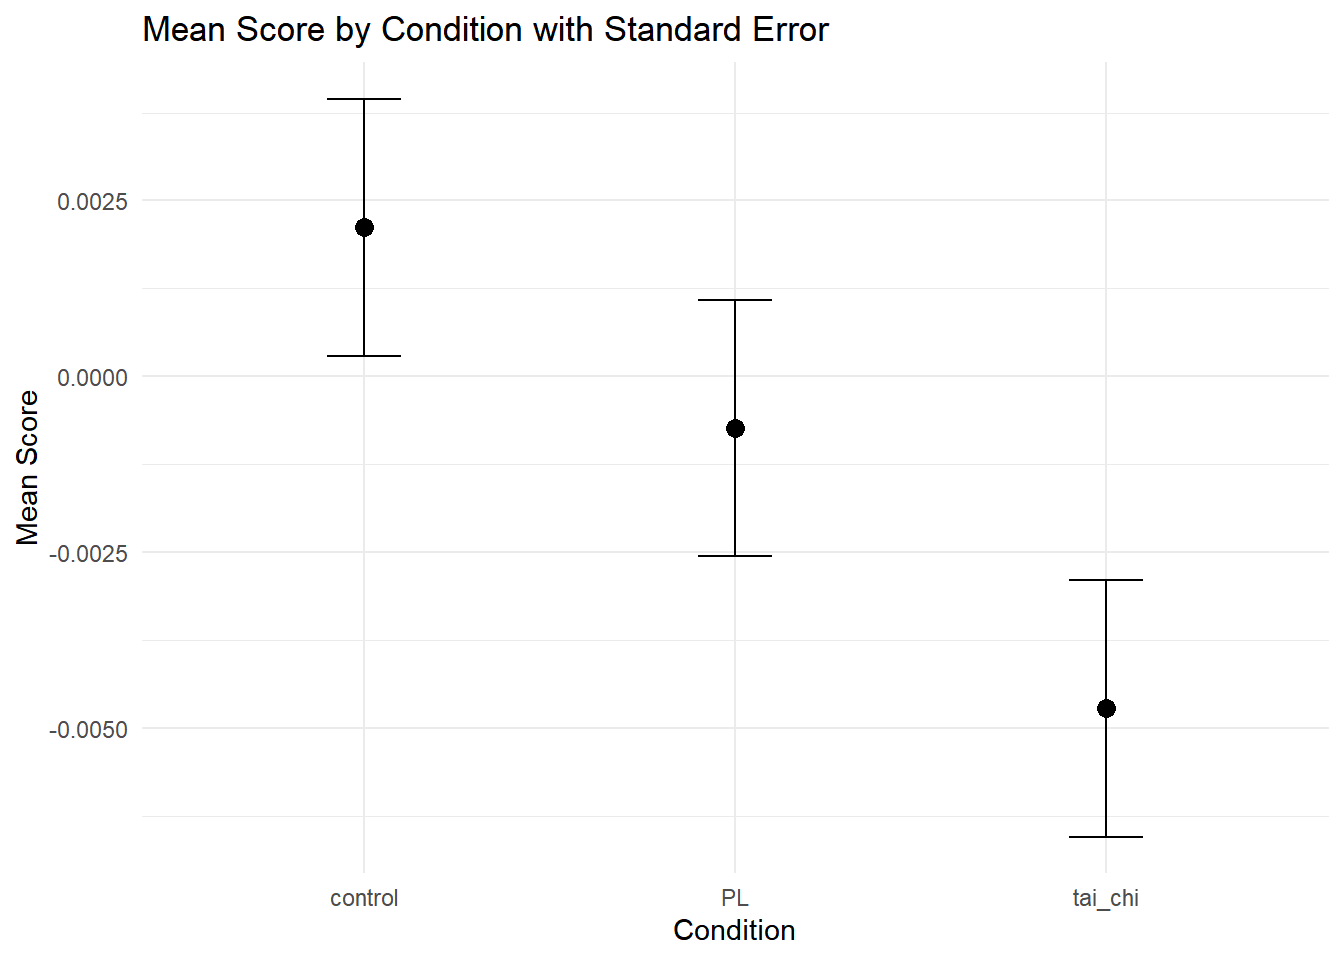
\includegraphics{3_p_values__lesson_files/figure-latex/unnamed-chunk-5-1.pdf}

\begin{Shaded}
\begin{Highlighting}[]
\FunctionTok{tibble}\NormalTok{(}\AttributeTok{p =} \FunctionTok{rbeta}\NormalTok{(}\AttributeTok{n =} \DecValTok{100000}\NormalTok{, }\AttributeTok{shape1 =} \DecValTok{1}\NormalTok{, }\AttributeTok{shape2 =} \DecValTok{1}\NormalTok{)) }\SpecialCharTok{|\textgreater{}}
  \FunctionTok{plot\_p\_values}\NormalTok{()}
\end{Highlighting}
\end{Shaded}

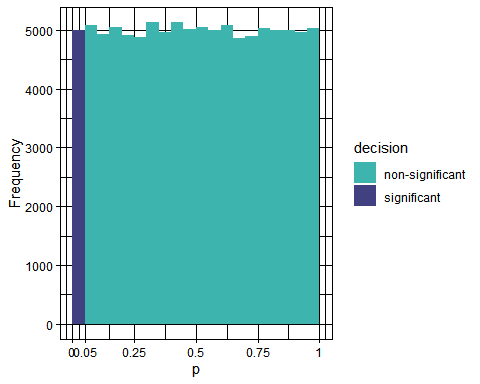
\includegraphics{3_p_values__lesson_files/figure-latex/unnamed-chunk-5-2.pdf}

\begin{Shaded}
\begin{Highlighting}[]
\FunctionTok{tibble}\NormalTok{(}\AttributeTok{p =} \FunctionTok{rbeta}\NormalTok{(}\AttributeTok{n =} \DecValTok{100000}\NormalTok{, }\AttributeTok{shape1 =} \DecValTok{1}\NormalTok{, }\AttributeTok{shape2 =} \DecValTok{5}\NormalTok{)) }\SpecialCharTok{|\textgreater{}}
  \FunctionTok{plot\_p\_values}\NormalTok{()}
\end{Highlighting}
\end{Shaded}

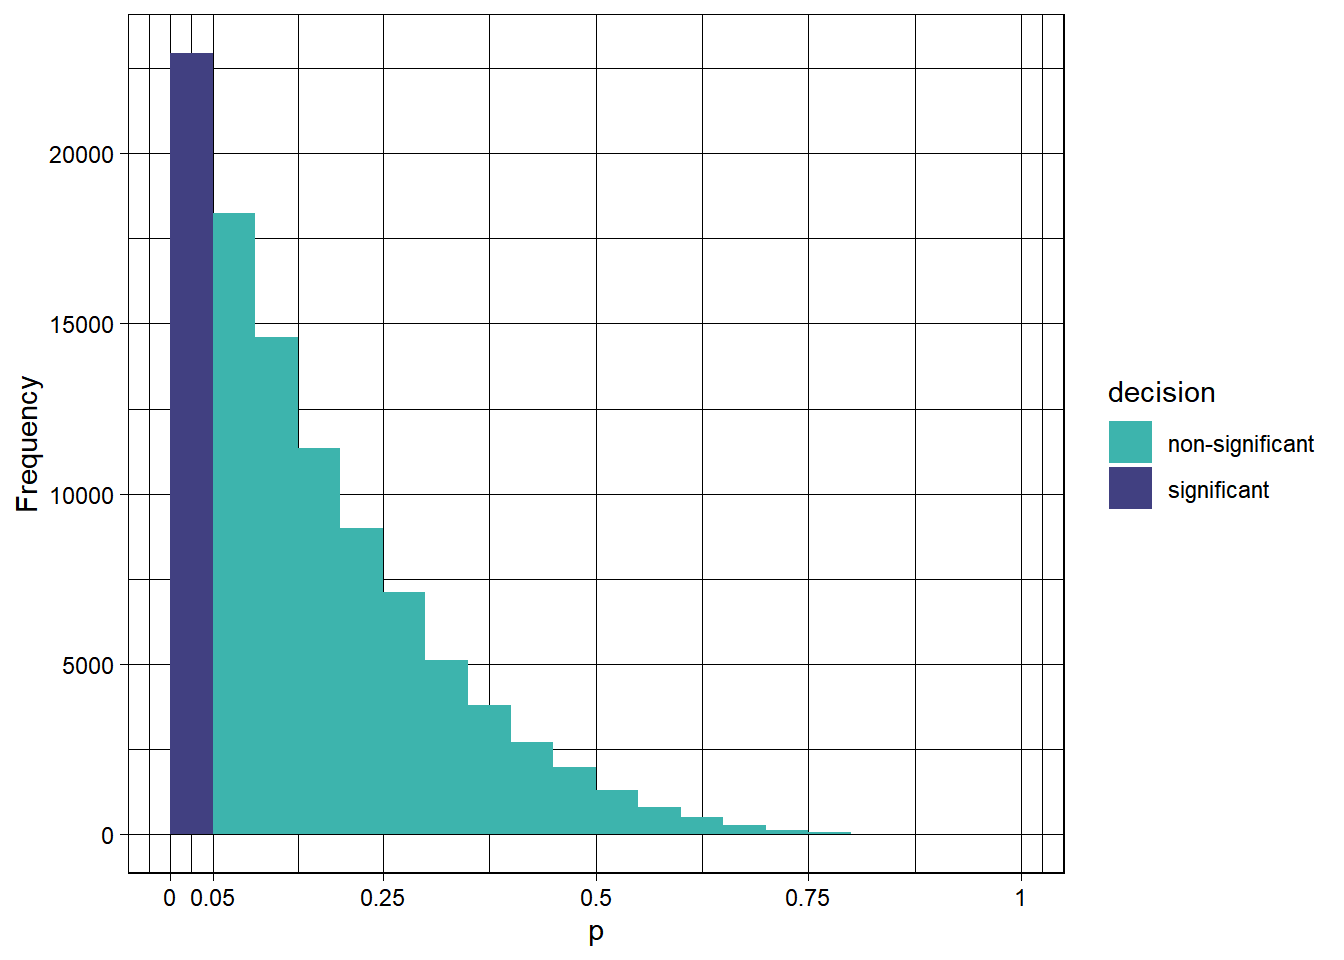
\includegraphics{3_p_values__lesson_files/figure-latex/unnamed-chunk-5-3.pdf}

\begin{Shaded}
\begin{Highlighting}[]
\FunctionTok{tibble}\NormalTok{(}\AttributeTok{p =} \FunctionTok{rbeta}\NormalTok{(}\AttributeTok{n =} \DecValTok{100000}\NormalTok{, }\AttributeTok{shape1 =} \FloatTok{0.1}\NormalTok{, }\AttributeTok{shape2 =} \DecValTok{5}\NormalTok{)) }\SpecialCharTok{|\textgreater{}}
  \FunctionTok{plot\_p\_values}\NormalTok{()}
\end{Highlighting}
\end{Shaded}

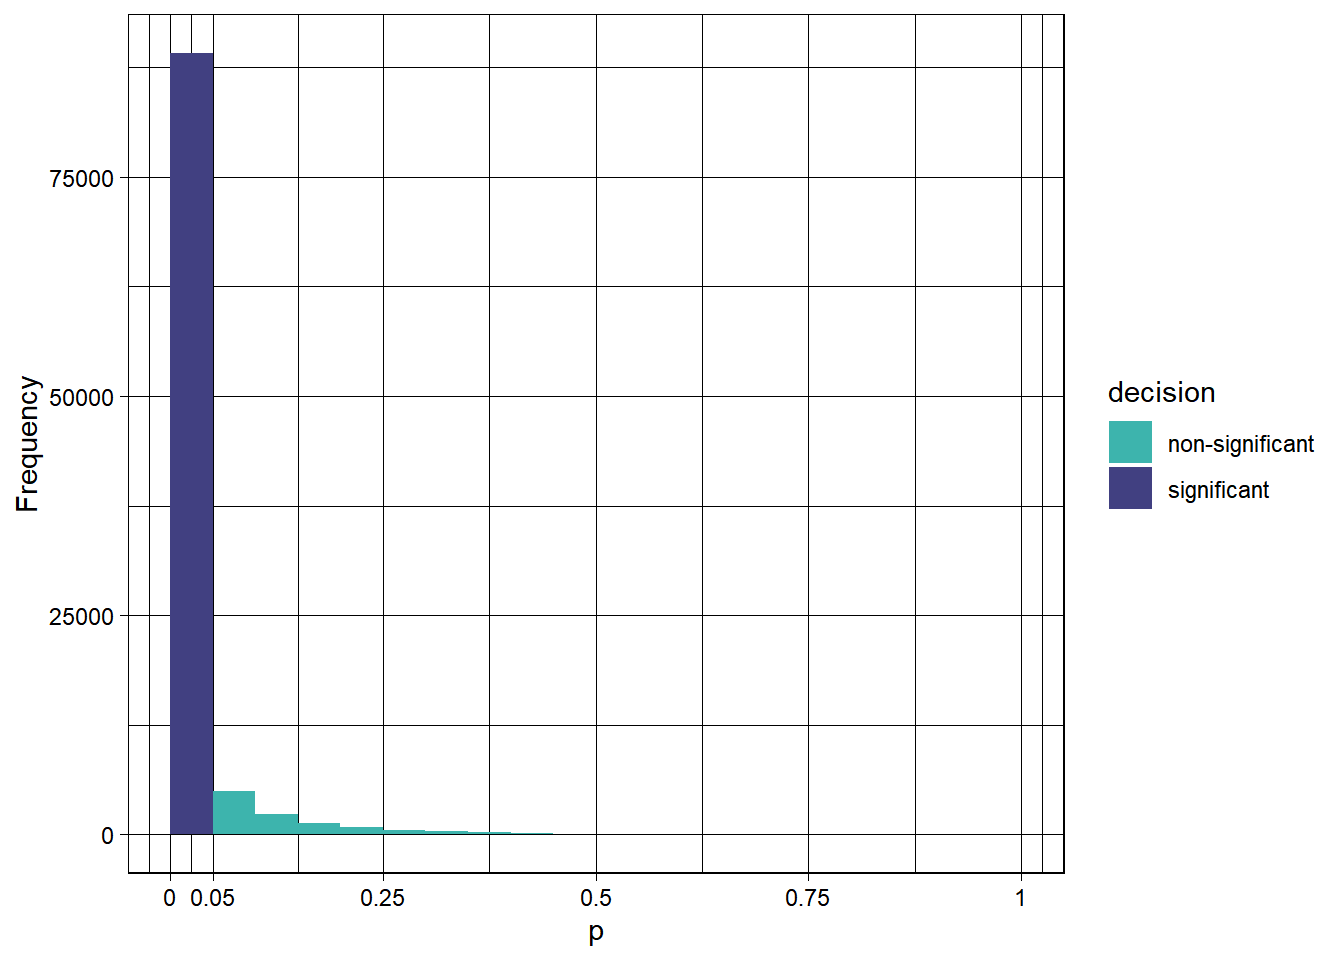
\includegraphics{3_p_values__lesson_files/figure-latex/unnamed-chunk-5-4.pdf}

\begin{itemize}
\tightlist
\item
  Again, these are not real \emph{p} values, just data sampled from a
  Beta distribution.
\end{itemize}

\hypertarget{the-distributions-of-p-values}{%
\section{\texorpdfstring{The distributions of \emph{p}
values}{The distributions of p values}}\label{the-distributions-of-p-values}}

Let's use (a) our understanding of how to construct a simulation {[}from
lesson 2{]} and (b) our function to plot data that are (or look like)
\emph{p} values to understand how \emph{p} values are distributed.

\hypertarget{simulate}{%
\subsection{Simulate}\label{simulate}}

The code for this simulation is copied from lesson 2 with few
modifications.

\begin{itemize}
\tightlist
\item
  No calculation of Cohen's \emph{d} as its not needed here.
\item
  Simulation parameters use a single sample size, but multiple true
  effect sizes including both null effects (Cohen's d = 0) and non-null
  effects (Cohen's d = 0.2, 0.5, 0.8, 1.0).
\end{itemize}

\begin{Shaded}
\begin{Highlighting}[]
\CommentTok{\# remove all objects from environment {-}{-}{-}{-}}
\CommentTok{\#rm(list = ls())}


\CommentTok{\# dependencies {-}{-}{-}{-}}
\CommentTok{\# repeated here for the sake of completeness }

\FunctionTok{library}\NormalTok{(tidyr)}
\FunctionTok{library}\NormalTok{(dplyr)}
\FunctionTok{library}\NormalTok{(forcats)}
\FunctionTok{library}\NormalTok{(readr)}
\FunctionTok{library}\NormalTok{(purrr) }
\FunctionTok{library}\NormalTok{(ggplot2)}
\FunctionTok{library}\NormalTok{(effsize)}
\FunctionTok{library}\NormalTok{(kableExtra)}
\end{Highlighting}
\end{Shaded}

\begin{verbatim}
## 
## Attache Paket: 'kableExtra'
\end{verbatim}

\begin{verbatim}
## Das folgende Objekt ist maskiert 'package:dplyr':
## 
##     group_rows
\end{verbatim}

\begin{Shaded}
\begin{Highlighting}[]
\FunctionTok{library}\NormalTok{(janitor)}
\end{Highlighting}
\end{Shaded}

\begin{verbatim}
## 
## Attache Paket: 'janitor'
\end{verbatim}

\begin{verbatim}
## Die folgenden Objekte sind maskiert von 'package:stats':
## 
##     chisq.test, fisher.test
\end{verbatim}

\begin{Shaded}
\begin{Highlighting}[]
\CommentTok{\# set the seed {-}{-}{-}{-}}
\CommentTok{\# for the pseudo random number generator to make results reproducible}
\FunctionTok{set.seed}\NormalTok{(}\DecValTok{123}\NormalTok{)}


\CommentTok{\# define data generating function {-}{-}{-}{-}}
\NormalTok{generate\_data }\OtherTok{\textless{}{-}} \ControlFlowTok{function}\NormalTok{(n\_control,}
\NormalTok{                          n\_intervention,}
\NormalTok{                          mean\_control,}
\NormalTok{                          mean\_intervention,}
\NormalTok{                          sd\_control,}
\NormalTok{                          sd\_intervention) \{}
  
\NormalTok{  data }\OtherTok{\textless{}{-}} 
    \FunctionTok{bind\_rows}\NormalTok{(}
      \FunctionTok{tibble}\NormalTok{(}\AttributeTok{condition =} \StringTok{"control"}\NormalTok{,}
             \AttributeTok{score =} \FunctionTok{rnorm}\NormalTok{(}\AttributeTok{n =}\NormalTok{ n\_control, }\AttributeTok{mean =}\NormalTok{ mean\_control, }\AttributeTok{sd =}\NormalTok{ sd\_control)),}
      \FunctionTok{tibble}\NormalTok{(}\AttributeTok{condition =} \StringTok{"intervention"}\NormalTok{,}
             \AttributeTok{score =} \FunctionTok{rnorm}\NormalTok{(}\AttributeTok{n =}\NormalTok{ n\_intervention, }\AttributeTok{mean =}\NormalTok{ mean\_intervention, }\AttributeTok{sd =}\NormalTok{ sd\_intervention))}
\NormalTok{    ) }\SpecialCharTok{|\textgreater{}}
    \CommentTok{\# control\textquotesingle{}s factor levels must be ordered so that intervention is the first level and control is the second}
    \CommentTok{\# this ensures that positive cohen\textquotesingle{}s d values refer to intervention \textgreater{} control and not the other way around.}
    \FunctionTok{mutate}\NormalTok{(}\AttributeTok{condition =} \FunctionTok{fct\_relevel}\NormalTok{(condition, }\StringTok{"intervention"}\NormalTok{, }\StringTok{"control"}\NormalTok{))}
  
  \FunctionTok{return}\NormalTok{(data)}
\NormalTok{\}}


\CommentTok{\# define data analysis function {-}{-}{-}{-}}
\NormalTok{analyse\_data }\OtherTok{\textless{}{-}} \ControlFlowTok{function}\NormalTok{(data) \{}

\NormalTok{  res\_t\_test }\OtherTok{\textless{}{-}} \FunctionTok{t.test}\NormalTok{(}\AttributeTok{formula =}\NormalTok{ score }\SpecialCharTok{\textasciitilde{}}\NormalTok{ condition, }
                       \AttributeTok{data =}\NormalTok{ data,}
                       \AttributeTok{var.equal =} \ConstantTok{FALSE}\NormalTok{,}
                       \AttributeTok{alternative =} \StringTok{"two.sided"}\NormalTok{)}
  
\NormalTok{  res }\OtherTok{\textless{}{-}} \FunctionTok{tibble}\NormalTok{(}\AttributeTok{p =}\NormalTok{ res\_t\_test}\SpecialCharTok{$}\NormalTok{p.value)}
  
  \FunctionTok{return}\NormalTok{(res)}
\NormalTok{\}}


\CommentTok{\# define experiment parameters {-}{-}{-}{-}}
\NormalTok{experiment\_parameters\_grid }\OtherTok{\textless{}{-}} \FunctionTok{expand\_grid}\NormalTok{(}
  \AttributeTok{n\_control =} \DecValTok{50}\NormalTok{,}
  \AttributeTok{n\_intervention =} \DecValTok{50}\NormalTok{,}
  \AttributeTok{mean\_control =} \DecValTok{0}\NormalTok{,}
  \AttributeTok{mean\_intervention =} \FunctionTok{c}\NormalTok{(}\FloatTok{0.0}\NormalTok{, }\FloatTok{0.1}\NormalTok{, }\FloatTok{0.2}\NormalTok{, }\FloatTok{0.5}\NormalTok{, }\FloatTok{0.8}\NormalTok{, }\FloatTok{1.0}\NormalTok{), }\CommentTok{\# only this differs meaningfully from the simulation in lesson 2: simulate data for a true effect size of 0 (null) and very small, small, medium, large, and very large Cohen\textquotesingle{}s d (alternative)}
  \AttributeTok{sd\_control =} \DecValTok{1}\NormalTok{,}
  \AttributeTok{sd\_intervention =} \DecValTok{1}\NormalTok{,}
  \AttributeTok{iteration =} \DecValTok{1}\SpecialCharTok{:}\DecValTok{10000} 
\NormalTok{)}


\CommentTok{\# run simulation {-}{-}{-}{-}}
\NormalTok{simulation }\OtherTok{\textless{}{-}} 
  \CommentTok{\# using the experiment parameters}
\NormalTok{  experiment\_parameters\_grid }\SpecialCharTok{|\textgreater{}}
  
  \CommentTok{\# generate data using the data generating function and the parameters relevant to data generation}
  \FunctionTok{mutate}\NormalTok{(}\AttributeTok{generated\_data =} \FunctionTok{pmap}\NormalTok{(}\FunctionTok{list}\NormalTok{(n\_control,}
\NormalTok{                                    n\_intervention,}
\NormalTok{                                    mean\_control,}
\NormalTok{                                    mean\_intervention,}
\NormalTok{                                    sd\_control,}
\NormalTok{                                    sd\_intervention),}
\NormalTok{                               generate\_data)) }\SpecialCharTok{|\textgreater{}}
  
  \CommentTok{\# apply the analysis function to the generated data using the parameters relevant to analysis}
  \FunctionTok{mutate}\NormalTok{(}\AttributeTok{analysis\_results =} \FunctionTok{pmap}\NormalTok{(}\FunctionTok{list}\NormalTok{(generated\_data),}
\NormalTok{                                 analyse\_data))}
  

\CommentTok{\# summarise simulation results over the iterations {-}{-}{-}{-}}
\NormalTok{simulation\_reshaped }\OtherTok{\textless{}{-}}\NormalTok{ simulation }\SpecialCharTok{|\textgreater{}}
  \CommentTok{\# convert \textasciigrave{}analysis\_results\textasciigrave{} nested{-}data{-}frame column to regular columns in the df. in this case, the p value.}
  \FunctionTok{unnest}\NormalTok{(analysis\_results) }\SpecialCharTok{|\textgreater{}}
  \CommentTok{\# label the true effect value}
  \FunctionTok{mutate}\NormalTok{(}\AttributeTok{true\_effect =} \FunctionTok{paste}\NormalTok{(}\StringTok{"Cohen\textquotesingle{}s d ="}\NormalTok{, mean\_intervention))}
\end{Highlighting}
\end{Shaded}

Results will be plotted in the next chunks.

\hypertarget{under-the-null-hypothesis}{%
\subsection{Under the null hypothesis}\label{under-the-null-hypothesis}}

I.e., the data generation (population) is an effect of zero.

\begin{Shaded}
\begin{Highlighting}[]
\NormalTok{simulation\_reshaped }\SpecialCharTok{|\textgreater{}}
  \CommentTok{\# using only the iterations where the population effect was from a true null population}
  \FunctionTok{filter}\NormalTok{(true\_effect }\SpecialCharTok{==} \StringTok{"Cohen\textquotesingle{}s d = 0"}\NormalTok{) }\SpecialCharTok{|\textgreater{}}
  \CommentTok{\# plot using our function}
  \FunctionTok{plot\_p\_values}\NormalTok{()}
\end{Highlighting}
\end{Shaded}

\includegraphics{3_p_values__lesson_files/figure-latex/unnamed-chunk-7-1.pdf}

\begin{Shaded}
\begin{Highlighting}[]
\NormalTok{simulation\_reshaped }\SpecialCharTok{|\textgreater{}}
  \FunctionTok{filter}\NormalTok{(true\_effect }\SpecialCharTok{==} \StringTok{"Cohen\textquotesingle{}s d = 0"}\NormalTok{) }\SpecialCharTok{|\textgreater{}}
  \FunctionTok{summarize}\NormalTok{(}\AttributeTok{false\_positive\_rate\_\_aka\_alpha =} \FunctionTok{mean}\NormalTok{(p }\SpecialCharTok{\textless{}}\NormalTok{ .}\DecValTok{05}\NormalTok{)) }\SpecialCharTok{|\textgreater{}}
  \FunctionTok{mutate\_if}\NormalTok{(is.numeric, janitor}\SpecialCharTok{::}\NormalTok{round\_half\_up, }\AttributeTok{digits =} \DecValTok{2}\NormalTok{)}
\end{Highlighting}
\end{Shaded}

\begin{verbatim}
## # A tibble: 1 x 1
##   false_positive_rate__aka_alpha
##                            <dbl>
## 1                           0.05
\end{verbatim}

\hypertarget{under-the-alternative-hypothesis}{%
\subsection{Under the alternative
hypothesis}\label{under-the-alternative-hypothesis}}

I.e., the data generation (population) is a non-zero effect.

We'll take just one non-zero effect size to start: the largest one
(Cohen's d = 1.0)

\begin{Shaded}
\begin{Highlighting}[]
\NormalTok{simulation\_reshaped }\SpecialCharTok{|\textgreater{}}
  \FunctionTok{filter}\NormalTok{(true\_effect }\SpecialCharTok{==} \StringTok{"Cohen\textquotesingle{}s d = 0.1"}\NormalTok{) }\SpecialCharTok{|\textgreater{}}
  \FunctionTok{plot\_p\_values}\NormalTok{()}
\end{Highlighting}
\end{Shaded}

\includegraphics{3_p_values__lesson_files/figure-latex/unnamed-chunk-8-1.pdf}

\begin{Shaded}
\begin{Highlighting}[]
\NormalTok{simulation\_reshaped }\SpecialCharTok{|\textgreater{}}
  \FunctionTok{filter}\NormalTok{(true\_effect }\SpecialCharTok{==} \StringTok{"Cohen\textquotesingle{}s d = 0.2"}\NormalTok{) }\SpecialCharTok{|\textgreater{}}
  \FunctionTok{plot\_p\_values}\NormalTok{()}
\end{Highlighting}
\end{Shaded}

\includegraphics{3_p_values__lesson_files/figure-latex/unnamed-chunk-8-2.pdf}

\begin{Shaded}
\begin{Highlighting}[]
\NormalTok{simulation\_reshaped }\SpecialCharTok{|\textgreater{}}
  \FunctionTok{filter}\NormalTok{(true\_effect }\SpecialCharTok{==} \StringTok{"Cohen\textquotesingle{}s d = 0.5"}\NormalTok{) }\SpecialCharTok{|\textgreater{}}
  \FunctionTok{plot\_p\_values}\NormalTok{()}
\end{Highlighting}
\end{Shaded}

\includegraphics{3_p_values__lesson_files/figure-latex/unnamed-chunk-8-3.pdf}

\begin{Shaded}
\begin{Highlighting}[]
\NormalTok{simulation\_reshaped }\SpecialCharTok{|\textgreater{}}
  \FunctionTok{filter}\NormalTok{(true\_effect }\SpecialCharTok{==} \StringTok{"Cohen\textquotesingle{}s d = 0.8"}\NormalTok{) }\SpecialCharTok{|\textgreater{}}
  \FunctionTok{plot\_p\_values}\NormalTok{()}
\end{Highlighting}
\end{Shaded}

\includegraphics{3_p_values__lesson_files/figure-latex/unnamed-chunk-8-4.pdf}

\begin{Shaded}
\begin{Highlighting}[]
\NormalTok{simulation\_reshaped }\SpecialCharTok{|\textgreater{}}
  \FunctionTok{filter}\NormalTok{(true\_effect }\SpecialCharTok{==} \StringTok{"Cohen\textquotesingle{}s d = 1"}\NormalTok{) }\SpecialCharTok{|\textgreater{}}
  \FunctionTok{plot\_p\_values}\NormalTok{()}
\end{Highlighting}
\end{Shaded}

\includegraphics{3_p_values__lesson_files/figure-latex/unnamed-chunk-8-5.pdf}

\begin{Shaded}
\begin{Highlighting}[]
\NormalTok{simulation\_reshaped }\SpecialCharTok{|\textgreater{}}
  \FunctionTok{filter}\NormalTok{(true\_effect }\SpecialCharTok{!=} \StringTok{"Cohen\textquotesingle{}s d = 0"}\NormalTok{) }\SpecialCharTok{|\textgreater{}}
  \FunctionTok{summarize}\NormalTok{(}\AttributeTok{true\_positive\_rate\_\_aka\_power =} \FunctionTok{mean}\NormalTok{(p }\SpecialCharTok{\textless{}}\NormalTok{ .}\DecValTok{05}\NormalTok{),}
            \AttributeTok{.by =}\NormalTok{ true\_effect) }\SpecialCharTok{|\textgreater{}}
  \FunctionTok{mutate\_if}\NormalTok{(is.numeric, janitor}\SpecialCharTok{::}\NormalTok{round\_half\_up, }\AttributeTok{digits =} \DecValTok{2}\NormalTok{)}
\end{Highlighting}
\end{Shaded}

\begin{verbatim}
## # A tibble: 5 x 2
##   true_effect     true_positive_rate__aka_power
##   <chr>                                   <dbl>
## 1 Cohen's d = 0.1                          0.07
## 2 Cohen's d = 0.2                          0.17
## 3 Cohen's d = 0.5                          0.7 
## 4 Cohen's d = 0.8                          0.98
## 5 Cohen's d = 1                            1
\end{verbatim}

\hypertarget{dance-of-the-p-values}{%
\section{\texorpdfstring{Dance of the \emph{p}
values}{Dance of the p values}}\label{dance-of-the-p-values}}

Let's look at the data a different way to understand what we mean by
``\emph{p} values are uniformly distributed under the null hypothesis''.

Uniform distributions mean that all variables in the range are just as
likely to occur.

For \emph{p} values, this means that \emph{p} values will dance back and
forth between 0 and 1 between a studies where the null hypothesis is
true (population effect is zero). I illustrate this blow by
\texttt{filter()}-ing only the true effect of 0 conditions, and taking
the first 150 iterations. You can see that between the iterations from
left to right, which represent independent experiments here, there is no
pattern among the \emph{p} values. Despite the true effect being zero, a
statistically significant result is still found sometimes, because
values of p = .01, .02, .03, .04 are just as probable as .48 or .97 or
any other.

\begin{Shaded}
\begin{Highlighting}[]
\NormalTok{simulation\_reshaped }\SpecialCharTok{|\textgreater{}}
  \FunctionTok{filter}\NormalTok{(true\_effect }\SpecialCharTok{==} \StringTok{"Cohen\textquotesingle{}s d = 0"}\NormalTok{) }\SpecialCharTok{|\textgreater{}}
  \FunctionTok{filter}\NormalTok{(iteration }\SpecialCharTok{\textless{}} \DecValTok{150}\NormalTok{) }\SpecialCharTok{|\textgreater{}}
  \FunctionTok{mutate}\NormalTok{(}\AttributeTok{decision =} \FunctionTok{ifelse}\NormalTok{(p }\SpecialCharTok{\textless{}}\NormalTok{ .}\DecValTok{05}\NormalTok{, }\StringTok{"significant"}\NormalTok{, }\StringTok{"non{-}significant"}\NormalTok{)) }\SpecialCharTok{|\textgreater{}}
  \FunctionTok{ggplot}\NormalTok{(}\FunctionTok{aes}\NormalTok{(iteration, p)) }\SpecialCharTok{+}
  \FunctionTok{geom\_line}\NormalTok{(}\AttributeTok{color =} \StringTok{"darkgrey"}\NormalTok{) }\SpecialCharTok{+}
  \FunctionTok{geom\_point}\NormalTok{(}\FunctionTok{aes}\NormalTok{(}\AttributeTok{color =}\NormalTok{ decision)) }\SpecialCharTok{+}
  \FunctionTok{scale\_color\_viridis\_d}\NormalTok{(}\AttributeTok{option =} \StringTok{"mako"}\NormalTok{, }\AttributeTok{begin =} \FloatTok{0.3}\NormalTok{, }\AttributeTok{end =} \FloatTok{0.7}\NormalTok{, }\AttributeTok{direction =} \SpecialCharTok{{-}}\DecValTok{1}\NormalTok{) }\SpecialCharTok{+}
  \FunctionTok{theme\_linedraw}\NormalTok{() }\SpecialCharTok{+}
  \FunctionTok{geom\_hline}\NormalTok{(}\AttributeTok{yintercept =} \FloatTok{0.05}\NormalTok{, }\AttributeTok{linetype =} \StringTok{"dashed"}\NormalTok{) }\SpecialCharTok{+}
  \FunctionTok{xlab}\NormalTok{(}\StringTok{"Experiment (iteration)"}\NormalTok{)}
\end{Highlighting}
\end{Shaded}

\includegraphics{3_p_values__lesson_files/figure-latex/unnamed-chunk-9-1.pdf}

\hypertarget{diagnosticity-of-a-given-p-value}{%
\section{\texorpdfstring{Diagnosticity of a given \emph{p}
value}{Diagnosticity of a given p value}}\label{diagnosticity-of-a-given-p-value}}

Of course, when you read the literature you don't have the advantage of
knowing whether the effect being studied is real or not. Instead, it
contains a mix or null and non-null effects - even when there is
absolutely no \emph{p}-hacking or publication bias.

This simulation assumes a range of true effects ranging from null to
medium, and an unknown mix of null and non-null effects. No
\emph{p}-hacking or publication bias involved - we'll come to this in a
future lesson. There's also no false positives due to violation of
assumptions.

\textbf{Re-run these chunks yourself a few times and see if you can
guess from looking at the first plot what the second plot will be made
up of. Eg., are most of the significant results true positives (non-null
effects) or false positives? Are most of the non-significant results
true null effects, or false-negatives?}

Remember that as well as assuming no \emph{p}-hacking or publication
bias, they also assume all assumptions have been met. False positive
rates go up if any of these are violated.

How the simulations are structured:

\begin{itemize}
\tightlist
\item
  Create a literature of 100 studies, studying different effects in the
  same broad domain.
\item
  In this literature, an unknown number of studies (k\_null) represent
  true null effects. This is done by sampling between 0 and 100 studies
  from the our existing simulations with a true effect of 0. The
  remaining number of studies (k\_nonnull) represent non-null effects of
  various sizes from very small to medium
\item
  The results from all the studies are then plotted together making only
  a significant vs.~non-significant distinction.
\end{itemize}

\textbf{Here, as in the real world, our job is to judge the findings in
a given literature only from the visible/published results, without ever
having access to their true status. How easy do you find it to whether a
given literature contains mostly real or null effects?}

\begin{Shaded}
\begin{Highlighting}[]
\NormalTok{k\_null }\OtherTok{\textless{}{-}} \FunctionTok{runif}\NormalTok{(}\AttributeTok{n =} \DecValTok{1}\NormalTok{, }\AttributeTok{min =} \DecValTok{0}\NormalTok{, }\AttributeTok{max =} \DecValTok{100}\NormalTok{) }\SpecialCharTok{|\textgreater{}} \FunctionTok{round}\NormalTok{(}\DecValTok{0}\NormalTok{)}
\NormalTok{k\_non\_null }\OtherTok{\textless{}{-}} \DecValTok{100} \SpecialCharTok{{-}}\NormalTok{ k\_null}

\CommentTok{\# simulate published literature by sampling from the existing simulation iterations}
\NormalTok{unbiased\_literature }\OtherTok{\textless{}{-}}
  \FunctionTok{bind\_rows}\NormalTok{(}
\NormalTok{    simulation\_reshaped }\SpecialCharTok{|\textgreater{}}
      \FunctionTok{filter}\NormalTok{(true\_effect }\SpecialCharTok{==} \StringTok{"Cohen\textquotesingle{}s d = 0"}\NormalTok{) }\SpecialCharTok{|\textgreater{}}
      \FunctionTok{sample\_n}\NormalTok{(k\_null),}
\NormalTok{    simulation\_reshaped }\SpecialCharTok{|\textgreater{}}
      \FunctionTok{filter}\NormalTok{(true\_effect }\SpecialCharTok{\%in\%} \FunctionTok{c}\NormalTok{(}\StringTok{"Cohen\textquotesingle{}s d = 0.1"}\NormalTok{, }\StringTok{"Cohen\textquotesingle{}s d = 0.2"}\NormalTok{, }\StringTok{"Cohen\textquotesingle{}s d = 0.5"}\NormalTok{)) }\SpecialCharTok{|\textgreater{}}
      \FunctionTok{sample\_n}\NormalTok{(k\_non\_null)}
\NormalTok{  ) }\SpecialCharTok{|\textgreater{}}
  \FunctionTok{mutate}\NormalTok{(}\AttributeTok{truth\_vs\_decision =} \FunctionTok{case\_when}\NormalTok{(true\_effect }\SpecialCharTok{==} \StringTok{"Cohen\textquotesingle{}s d = 0"} \SpecialCharTok{\&}\NormalTok{ p }\SpecialCharTok{\textgreater{}=}\NormalTok{ .}\DecValTok{05} \SpecialCharTok{\textasciitilde{}} \StringTok{"True negatives"}\NormalTok{,}
\NormalTok{                                       true\_effect }\SpecialCharTok{==} \StringTok{"Cohen\textquotesingle{}s d = 0"} \SpecialCharTok{\&}\NormalTok{ p }\SpecialCharTok{\textless{}}\NormalTok{  .}\DecValTok{05} \SpecialCharTok{\textasciitilde{}} \StringTok{"False positives"}\NormalTok{,}
\NormalTok{                                       true\_effect }\SpecialCharTok{!=} \StringTok{"Cohen\textquotesingle{}s d = 0"} \SpecialCharTok{\&}\NormalTok{ p }\SpecialCharTok{\textgreater{}=}\NormalTok{ .}\DecValTok{05} \SpecialCharTok{\textasciitilde{}} \StringTok{"False negatives"}\NormalTok{,}
\NormalTok{                                       true\_effect }\SpecialCharTok{!=} \StringTok{"Cohen\textquotesingle{}s d = 0"} \SpecialCharTok{\&}\NormalTok{ p }\SpecialCharTok{\textless{}}\NormalTok{  .}\DecValTok{05} \SpecialCharTok{\textasciitilde{}} \StringTok{"True positives"}\NormalTok{))}
\end{Highlighting}
\end{Shaded}

\hypertarget{published-literature}{%
\subsection{Published literature}\label{published-literature}}

\begin{Shaded}
\begin{Highlighting}[]
\NormalTok{unbiased\_literature }\SpecialCharTok{|\textgreater{}}
  \FunctionTok{plot\_p\_values}\NormalTok{()}
\end{Highlighting}
\end{Shaded}

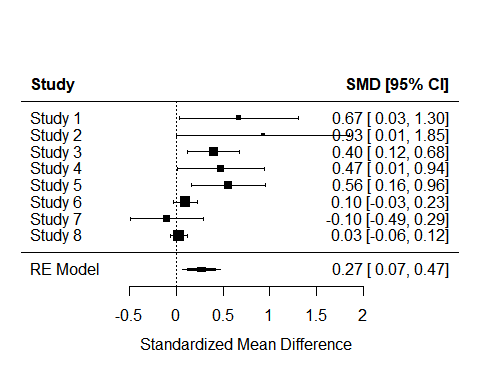
\includegraphics{3_p_values__lesson_files/figure-latex/unnamed-chunk-11-1.pdf}

\hypertarget{true-effects-underlying-the-published-literature}{%
\section{True effects underlying the published
literature}\label{true-effects-underlying-the-published-literature}}

(unknowable in the real world)

The table also calculates the ``false discovery rate'' and the ``missed
discovery rate'' within each literature. These represent the proportion
of all positives that are false positives, and the proportion of all
negatives that are true negatives.

\begin{Shaded}
\begin{Highlighting}[]
\NormalTok{unbiased\_literature }\SpecialCharTok{|\textgreater{}}
  \FunctionTok{ggplot}\NormalTok{(}\FunctionTok{aes}\NormalTok{(p, }\AttributeTok{fill =}\NormalTok{ truth\_vs\_decision)) }\SpecialCharTok{+}
  \FunctionTok{geom\_histogram}\NormalTok{(}\AttributeTok{binwidth =} \FloatTok{0.05}\NormalTok{, }\AttributeTok{boundary =} \DecValTok{0}\NormalTok{) }\SpecialCharTok{+}
  \FunctionTok{scale\_fill\_viridis\_d}\NormalTok{(}\AttributeTok{option =} \StringTok{"magma"}\NormalTok{, }\AttributeTok{begin =} \FloatTok{0.2}\NormalTok{, }\AttributeTok{end =} \FloatTok{0.9}\NormalTok{, }\AttributeTok{direction =} \SpecialCharTok{{-}}\DecValTok{1}\NormalTok{) }\SpecialCharTok{+}
  \FunctionTok{scale\_x\_continuous}\NormalTok{(}\AttributeTok{labels =} \FunctionTok{c}\NormalTok{(}\DecValTok{0}\NormalTok{, }\FloatTok{0.05}\NormalTok{, }\FloatTok{0.25}\NormalTok{, }\FloatTok{0.50}\NormalTok{, }\FloatTok{0.75}\NormalTok{, }\FloatTok{1.0}\NormalTok{),}
                     \AttributeTok{breaks =} \FunctionTok{c}\NormalTok{(}\DecValTok{0}\NormalTok{, }\FloatTok{0.05}\NormalTok{, }\FloatTok{0.25}\NormalTok{, }\FloatTok{0.50}\NormalTok{, }\FloatTok{0.75}\NormalTok{, }\FloatTok{1.0}\NormalTok{), }
                     \AttributeTok{limits =} \FunctionTok{c}\NormalTok{(}\DecValTok{0}\NormalTok{, }\DecValTok{1}\NormalTok{)) }\SpecialCharTok{+}
  \FunctionTok{theme\_linedraw}\NormalTok{() }\SpecialCharTok{+}
  \FunctionTok{ylab}\NormalTok{(}\StringTok{"Frequency"}\NormalTok{)}
\end{Highlighting}
\end{Shaded}

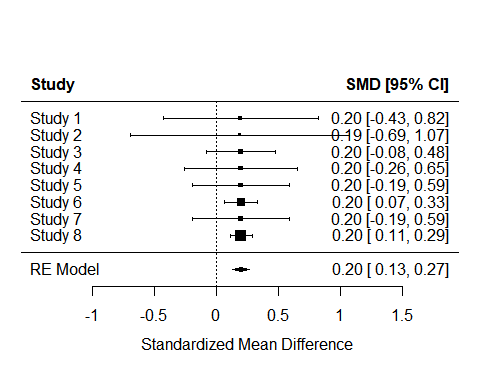
\includegraphics{3_p_values__lesson_files/figure-latex/unnamed-chunk-12-1.pdf}

\begin{Shaded}
\begin{Highlighting}[]
\NormalTok{unbiased\_literature }\SpecialCharTok{|\textgreater{}}
  \FunctionTok{count}\NormalTok{(truth\_vs\_decision) }\SpecialCharTok{|\textgreater{}}
  \FunctionTok{pivot\_wider}\NormalTok{(}\AttributeTok{names\_from =}\NormalTok{ truth\_vs\_decision, }
              \AttributeTok{values\_from =}\NormalTok{ n) }\SpecialCharTok{|\textgreater{}}
  \FunctionTok{mutate}\NormalTok{(}\StringTok{\textasciigrave{}}\AttributeTok{False discovery rate}\StringTok{\textasciigrave{}} \OtherTok{=} \FunctionTok{round\_half\_up}\NormalTok{(}\StringTok{\textasciigrave{}}\AttributeTok{False positives}\StringTok{\textasciigrave{}} \SpecialCharTok{/}\NormalTok{ (}\StringTok{\textasciigrave{}}\AttributeTok{False positives}\StringTok{\textasciigrave{}} \SpecialCharTok{+} \StringTok{\textasciigrave{}}\AttributeTok{True positives}\StringTok{\textasciigrave{}}\NormalTok{), }\AttributeTok{digits =} \DecValTok{2}\NormalTok{),}
         \StringTok{\textasciigrave{}}\AttributeTok{Missed discovery rate}\StringTok{\textasciigrave{}} \OtherTok{=} \FunctionTok{round\_half\_up}\NormalTok{(}\StringTok{\textasciigrave{}}\AttributeTok{False negatives}\StringTok{\textasciigrave{}} \SpecialCharTok{/}\NormalTok{ (}\StringTok{\textasciigrave{}}\AttributeTok{False negatives}\StringTok{\textasciigrave{}} \SpecialCharTok{+} \StringTok{\textasciigrave{}}\AttributeTok{True negatives}\StringTok{\textasciigrave{}}\NormalTok{), }\AttributeTok{digits =} \DecValTok{2}\NormalTok{)) }\SpecialCharTok{|\textgreater{}}
  \CommentTok{\#pivot\_longer(cols = everything()) |\textgreater{}}
  \CommentTok{\#mutate\_if(is.numeric, janitor::round\_half\_up, digits = 2) |\textgreater{}}
  \FunctionTok{kable}\NormalTok{() }\SpecialCharTok{|\textgreater{}}
  \FunctionTok{kable\_classic}\NormalTok{(}\AttributeTok{full\_width =} \ConstantTok{FALSE}\NormalTok{)}
\end{Highlighting}
\end{Shaded}

\begin{longtable}[t]{rrrrrr}
\toprule
False negatives & False positives & True negatives & True positives & False discovery rate & Missed discovery rate\\
\midrule
15 & 3 & 73 & 9 & 0.25 & 0.17\\
\bottomrule
\end{longtable}

\hypertarget{session-info}{%
\section{Session info}\label{session-info}}

\begin{Shaded}
\begin{Highlighting}[]
\FunctionTok{sessionInfo}\NormalTok{()}
\end{Highlighting}
\end{Shaded}

\begin{verbatim}
## R version 4.3.2 (2023-10-31 ucrt)
## Platform: x86_64-w64-mingw32/x64 (64-bit)
## Running under: Windows 11 x64 (build 22631)
## 
## Matrix products: default
## 
## 
## locale:
## [1] LC_COLLATE=German_Switzerland.utf8  LC_CTYPE=German_Switzerland.utf8   
## [3] LC_MONETARY=German_Switzerland.utf8 LC_NUMERIC=C                       
## [5] LC_TIME=German_Switzerland.utf8    
## 
## time zone: Europe/Zurich
## tzcode source: internal
## 
## attached base packages:
## [1] stats     graphics  grDevices utils     datasets  methods   base     
## 
## other attached packages:
##  [1] janitor_2.2.0    kableExtra_1.4.0 effsize_0.8.1    lubridate_1.9.3 
##  [5] forcats_1.0.0    stringr_1.5.1    dplyr_1.1.4      purrr_1.0.2     
##  [9] readr_2.1.5      tidyr_1.3.1      tibble_3.2.1     ggplot2_3.5.0   
## [13] tidyverse_2.0.0 
## 
## loaded via a namespace (and not attached):
##  [1] utf8_1.2.4        generics_0.1.3    xml2_1.3.6        stringi_1.8.3    
##  [5] hms_1.1.3         digest_0.6.35     magrittr_2.0.3    evaluate_0.23    
##  [9] grid_4.3.2        timechange_0.3.0  fastmap_1.1.1     fansi_1.0.6      
## [13] viridisLite_0.4.2 scales_1.3.0      cli_3.6.2         rlang_1.1.3      
## [17] munsell_0.5.0     withr_3.0.0       yaml_2.3.8        tools_4.3.2      
## [21] tzdb_0.4.0        colorspace_2.1-0  vctrs_0.6.5       R6_2.5.1         
## [25] lifecycle_1.0.4   snakecase_0.11.1  pkgconfig_2.0.3   pillar_1.9.0     
## [29] gtable_0.3.4      glue_1.7.0        systemfonts_1.0.6 xfun_0.42        
## [33] tidyselect_1.2.1  highr_0.10        rstudioapi_0.15.0 knitr_1.45       
## [37] farver_2.1.1      htmltools_0.5.7   rmarkdown_2.26    svglite_2.1.3    
## [41] labeling_0.4.3    compiler_4.3.2
\end{verbatim}

\end{document}
